\documentclass{article}
\usepackage{nirav-ma403}

\newcommand{\myname}{Nirav Bhattad (23B3307)}
\newcommand{\topicname}{EE659: Assignment 5}

\begin{document}

\thispagestyle{empty}

\titleBC
% \tableofcontents
% \clearpage

\begin{question*}[1]
	Let \( f(\mathbf{x}) \), where \( \mathbf{x} = \begin{bmatrix} x_1 & x_2 \end{bmatrix}^\top \in \mathbb{R}^2 \), be given by

    \[
        f(\mathbf{x}) = 5x_1^2 + x_2^2 + 2x_1 x_2 - 3x_1 - x_2.
    \]

    \begin{enumerate}[label=(\alph*)]
        \item Express \( f(\mathbf{x}) \) in the form of \( f(\mathbf{x}) = \frac{1}{2} \mathbf{x}^\top Q \mathbf{x} - \mathbf{x}^\top \mathbf{b} \).
        \item Find the minimizer of \( f \) using the conjugate gradient algorithm. Use a starting point of \( \mathbf{x}^{(0)} = (0, 0)^\top\), where \( \mathbf{x} = \begin{bmatrix} x_1 & x_2 \end{bmatrix}^\top \).
    \end{enumerate}
\end{question*}

\begin{proof}
We begin by identifying the quadratic terms and linear terms in the function \( f(\mathbf{x}) \).

Quadratic terms: \\
\begin{itemize}
\item The coefficient of \( x_1^2 \) is \( 5 \), so \( Q_{11} = 10 \) (since we have a factor of \( \frac{1}{2} \) in the quadratic form).
\item The coefficient of \( x_2^2 \) is \( 1 \), so \( Q_{22} = 2 \).
\item The coefficient of \( x_1 x_2 \) is \( 2 \), so \( Q_{12} = Q_{21} = 1 \).
\end{itemize}

Thus, the matrix \( Q \) is:

\[
Q = \begin{bmatrix} 10 & 1 \\ 1 & 2 \end{bmatrix}.
\]

Linear terms: \\
The linear terms are \( -3x_1 \) and \( -x_2 \). Hence, the vector \( \mathbf{b} \) is:

\[
\mathbf{b} = \begin{bmatrix} 3 \\ 1 \end{bmatrix}.
\]

Therefore, we can express the function as:

\[
f(\mathbf{x}) = \frac{1}{2} \mathbf{x}^\top \begin{bmatrix} 10 & 1 \\ 1 & 2 \end{bmatrix} \mathbf{x} - \mathbf{x}^\top \begin{bmatrix} 3 & 1 \end{bmatrix}.
\]

For the second part, we resort to Python.

\begin{lstlisting}[language=Python]
import numpy as np

Q = np.array([[10, 1], [1, 2]])
b = np.array([3, 1])

def conjugate_gradient(Q, b, x0=None, tol=1e-9, max_iter=1000):
    if x0 is None:
        x = np.zeros_like(b)  
    else:
        x = x0
    r = b - np.dot(Q, x)  
    p = r.copy()  
    rs_old = np.dot(r, r)
    
    for i in range(max_iter):
        Ap = np.dot(Q, p)
        alpha = rs_old / np.dot(p, Ap)
        x = x + alpha * p
        r = r - alpha * Ap
        rs_new = np.dot(r, r)
        
        if np.sqrt(rs_new) < tol:
            break
        
        beta = rs_new / rs_old
        p = r + beta * p
        rs_old = rs_new
    
    return x, i + 1  

x0 = np.zeros(2)

solution, iterations = conjugate_gradient(Q, b, x0)
print(f"Solution: {solution}")
print(f"Iterations: {iterations}")
\end{lstlisting}

We get the results as shown below:

\begin{figure}[H]
    \centering
    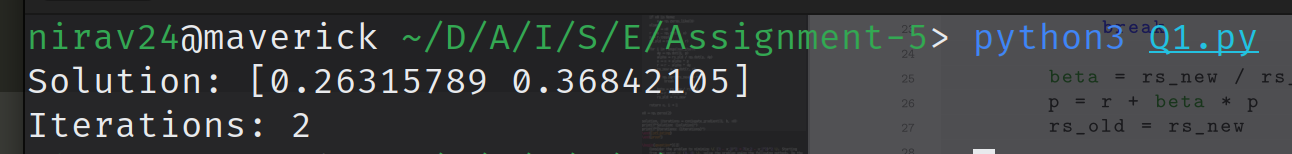
\includegraphics[width=0.8\textwidth]{Images/Q1.png}
\end{figure}
\end{proof}

\begin{question*}[2]
    Consider the problem to minimize \( (3 - x_1)^2 + 7(x_2 - x_1^2)^2 \). Starting from the point \( (0, 0) \), solve the problem using the following methods. Do the methods converge to the same point? If not, explain.

    \begin{enumerate}[label=(\alph*)]
        \item The method of Fletcher and Reeves.
        \item The method of Davidon-Fletcher-Powell.
    \end{enumerate}
\end{question*}

\begin{proof}[(a)]
We solve this numerically using Python. 
\begin{lstlisting}[language=Python]
import numpy as np

def f(x):
    x1, x2 = x
    return (3 - x1)**2 + 7 * (x2 - x1**2)**2

def grad_f(x):
    x1, x2 = x
    df_dx1 = -2 * (3 - x1) - 14 * (x2 - x1**2) * 2 * x1
    df_dx2 = 14 * (x2 - x1**2)
    
    grad = np.array([df_dx1, df_dx2])
    grad = np.clip(grad, -10, 10)
    
    return grad

def fletcher_reeves_method(x0, tol=1e-6, max_iter=1000):
    x = x0
    grad = grad_f(x)
    p = -grad  
    iter_count = 0
    alpha = 0.01
    
    while np.linalg.norm(grad) > tol and iter_count < max_iter:
        x = x + alpha * p
        new_grad = grad_f(x)
        
        beta = np.dot(new_grad, new_grad) / np.dot(grad, grad)
        p = -new_grad + beta * p
        
        grad = new_grad
        iter_count += 1
        
        if np.any(np.isnan(grad)) or np.any(np.isinf(grad)):
            print("Gradient became NaN or Inf!")
            break
    
    return x, iter_count

x0 = np.array([0.0, 0.0])

solution_fletcher_reeves, iterations_fletcher_reeves = fletcher_reeves_method(x0)
print(f"Fletcher and Reeves solution: {solution_fletcher_reeves}")
print(f"Iterations: {iterations_fletcher_reeves}")
\end{lstlisting}
\end{proof}

\begin{proof}[(b)]
We solve this numerically using Python. 
\begin{lstlisting}[language=Python]
import numpy as np

def f(x):
    x1, x2 = x
    return (3 - x1)**2 + 7 * (x2 - x1**2)**2

def grad_f(x):
    x1, x2 = x
    df_dx1 = -2 * (3 - x1) - 14 * (x2 - x1**2) * 2 * x1
    df_dx2 = 14 * (x2 - x1**2)
    return np.array([df_dx1, df_dx2])

def dfp_method(x0, tol=1e-6, max_iter=1000):
    x = x0
    grad = grad_f(x)
    H = np.eye(len(x))
    iter_count = 0
    
    while np.linalg.norm(grad) > tol and iter_count < max_iter:
        p = -np.dot(H, grad)  # search direction
        alpha = 0.01  
        x_new = x + alpha * p
        grad_new = grad_f(x_new)
        
        s = x_new - x
        y = grad_new - grad
        
        H = H + np.outer(y, y) / np.dot(y, s) - np.dot(np.dot(H, np.outer(s, s)), H) / np.dot(s, np.dot(H, s))
        
        x = x_new
        grad = grad_new
        iter_count += 1
    
    return x, iter_count

x0 = np.array([0.0, 0.0])

solution_dfp, iterations_dfp = dfp_method(x0)
print(f"Davidon-Fletcher-Powell solution: {solution_dfp}")
print(f"Iterations: {iterations_dfp}")
\end{lstlisting}
\end{proof}

\begin{question*}[3]
    Consider the problem

    \[
    \text{minimize} \quad x_1^2 + x_2^2 + x_3^2 + x_4^2 - 2x_1 - 3x_4
    \]
    subject to
    \[
    2x_1 + x_2 + x_3 + 4x_4 = 7,
    \]
    \[
    x_1 + x_2 + 3x_3 + x_4 = 6,
    \]
    \[
    x_i \geq 0, \quad i = 1, 2, 3, 4
    \]

    \begin{enumerate}[label=(\alph*)]
        \item Solve the problem using any optimization technique learned.
        \item Suppose the given initial guess is \( \mathbf{x} = (2, 2, 1, 0) \), perform two iterations of the gradient projection method and comment on the directions obtained.
    \end{enumerate}
\end{question*}

\begin{proof}
    We will solve this problem using the method of Lagrange multipliers. The objective function is:
    \[
    f(x_1, x_2, x_3, x_4) = x_1^2 + x_2^2 + x_3^2 + x_4^2 - 2x_1 - 3x_4
    \]
    The gradient of \( f(x) \) is:
    \[
    \nabla f(x) = \left( \frac{\partial f}{\partial x_1}, \frac{\partial f}{\partial x_2}, \frac{\partial f}{\partial x_3}, \frac{\partial f}{\partial x_4} \right)
    \]
    We compute each partial derivative:
    \[
    \frac{\partial f}{\partial x_1} = 2x_1 - 2, \quad \frac{\partial f}{\partial x_2} = 2x_2, \quad \frac{\partial f}{\partial x_3} = 2x_3, \quad \frac{\partial f}{\partial x_4} = 2x_4 - 3
    \]
    Thus, the gradient is:
    \[
    \nabla f(x) = \left( 2x_1 - 2, 2x_2, 2x_3, 2x_4 - 3 \right)
    \]
    The constraints are:
    \[
    2x_1 + x_2 + x_3 + 4x_4 = 7,
    \]
    \[
    x_1 + x_2 + 3x_3 + x_4 = 6
    \]
    We form the Lagrangian:
    \[
    \mathcal{L}(x_1, x_2, x_3, x_4, \lambda_1, \lambda_2) = f(x_1, x_2, x_3, x_4) + \lambda_1 (2x_1 + x_2 + x_3 + 4x_4 - 7) + \lambda_2 (x_1 + x_2 + 3x_3 + x_4 - 6)
    \]
    We need to solve the system:

    \[
    \begin{aligned}
    2x_1 - 2 + 2\lambda_1 + \lambda_2 &= 0 \\
    2x_2 + \lambda_1 + \lambda_2 &= 0 \\
    2x_3 + \lambda_1 + 3\lambda_2 &= 0 \\
    2x_4 - 3 + 4\lambda_1 + \lambda_2 &= 0 \\
    2x_1 + x_2 + x_3 + 4x_4 &= 7 \\
    x_1 + x_2 + 3x_3 + x_4 &= 6
    \end{aligned}
    \]

    By solving this system, we obtain the values of \( x_1, x_2, x_3, x_4, \lambda_1, \lambda_2 \).

\begin{lstlisting}[language=Python]
import numpy as np
from scipy.linalg import solve

A = np.array([
    [2, 0, 0, 0, 2, 1],
    [0, 2, 0, 0, 1, 1],
    [0, 0, 2, 0, 1, 3],
    [0, 0, 0, 2, 4, 1],
    [2, 1, 1, 4, 0, 0],
    [1, 1, 3, 1, 0, 0]
])

b = np.array([2, 0, 0, 3, 7, 6])

solution = solve(A, b)

x1, x2, x3, x4, lambda1, lambda2 = solution
print(f"x1 = {x1}, x2 = {x2}, x3 = {x3}, x4 = {x4}, lambda1 = {lambda1}, lambda2 = {lambda2}")
\end{lstlisting}

\begin{figure}[H]
    \centering
    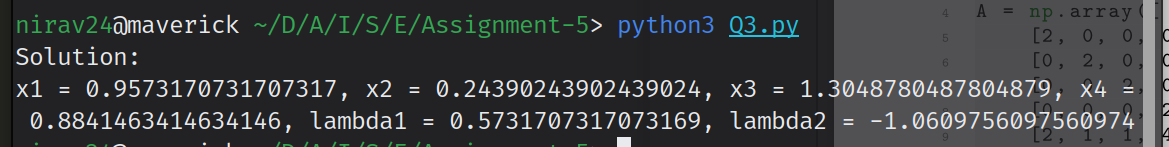
\includegraphics[width=0.8\textwidth]{Images/Q3.png}
\end{figure}
\end{proof}

% \clearpage

\begin{question*}[4]
    Consider the problem:

    \[
    \text{minimize} \quad f(x) = x^{\frac{4}{3}}
    \]

    Note that \( 0 \) is the global minimizer of \( f \).

    \begin{enumerate}[label=(\alph*)]
        \item Write down the algorithm for Newton's method applied to this problem.
        
        \item Show that as long as the starting point is not \( 0 \), the algorithm in part (a) does not converge to \( 0 \), no matter how close to \( 0 \) we start.
    \end{enumerate}
\end{question*}

We are given the function \( f(x) = x^{\frac{4}{3}} \) and need to apply Newton's method for minimization. The general update rule for Newton's method is:
\[
x_{k+1} = x_k - \frac{f'(x_k)}{f''(x_k)}
\]
First, we compute the first and second derivatives of the function \( f(x) \):
\[
f'(x) = \frac{d}{dx}\left(x^{\frac{4}{3}}\right) = \frac{4}{3} x^{\frac{1}{3}}
\]
\[
f''(x) = \frac{d}{dx}\left(\frac{4}{3} x^{\frac{1}{3}}\right) = \frac{4}{9} x^{-\frac{2}{3}}
\]
Now, applying the Newton's method update rule:
\[
x_{k+1} = x_k - \frac{\frac{4}{3} x_k^{\frac{1}{3}}}{\frac{4}{9} x_k^{-\frac{2}{3}}}
\]
Simplifying the expression:
\[
x_{k+1} = x_k - 3x_k
\]
\[
x_{k+1} = -2x_k
\]
Thus, the algorithm for Newton's method applied to this problem is:
\[
x_{k+1} = -2x_k
\]
We now analyze the convergence behavior of the algorithm. The update rule derived earlier is:
\[
x_{k+1} = -2x_k
\]
This means that at each iteration, the value of \( x_k \) is multiplied by \(-2\). Therefore, the sequence \( \{x_k\} \) evolves as follows:
\[
x_0, \quad x_1 = -2x_0, \quad x_2 = -2x_1 = 4x_0, \quad x_3 = -2x_2 = -8x_0, \quad \dots
\]
So, the sequence alternates between multiplying the previous value by \(-2\). As we can observe, no matter how small \( |x_0| \) is (as long as \( x_0 \neq 0 \)), the values of \( x_k \) will either grow or shrink but will never approach zero. Specifically, the magnitude of \( x_k \) grows exponentially (in absolute value) because each iteration multiplies the previous value by $2$. \\

Therefore, as long as the starting point \( x_0 \neq 0 \), the sequence will not converge to \( 0 \); rather, it will diverge. Thus, the algorithm does \textbf{not} converge to \( 0 \), regardless of how close the starting point is to zero, as long as \( x_0 \neq 0 \).

% \clearpage

\begin{question*}[5]
    Solve the problem to minimize 
    \[
    2x_1 + 3x_2^2 + e^{2x_1^2 + x_2^2}
    \]
    starting with the point \( (1, 0) \), and using both the Fletcher and Reeves conjugate gradient method and the Broyden-Fletcher-Goldfarb-Shanno (BFGS) quasi-Newton method.
\end{question*}

We use python to solve the above problem. The code is as follows:

\begin{lstlisting}[language=Python]
import numpy as np
from scipy.optimize import minimize

def objective(x):
    x1, x2 = x
    exp_term = np.exp(np.clip(2 * x1**2 + x2**2, -50, 50))
    return 2 * x1 + 3 * x2**2 + exp_term

def gradient(x):
    x1, x2 = x
    exp_term = np.exp(np.clip(2 * x1**2 + x2**2, -50, 50)) 
    grad_x1 = 2 + 4 * x1 * exp_term
    grad_x2 = 6 * x2 + 2 * x2 * exp_term
    return np.array([grad_x1, grad_x2])

def fletcher_reeves_cg(func, grad, x0, tol=1e-6, max_iter=100):
    x = x0
    g = grad(x)  
    d = -g  
    for i in range(max_iter):
        g = grad(x)
        step_size = 0.1 
        x_new = x + step_size * d
        g_new = grad(x_new)
        
        if np.linalg.norm(g_new) < tol:
            print(f"Converged at iteration {i}")
            break
        
        beta = np.dot(g_new, g_new) / np.dot(g, g)
        d = -g_new + beta * d
        x = x_new
        g = g_new
        
    return x, func(x)

def bfgs(func, grad, x0, tol=1e-6, max_iter=50, epsilon=1e-8):
    x = x0
    n = len(x)
    
    H = np.eye(n)
    
    f = func(x)
    g = grad(x)
    
    for _ in range(max_iter):
        p = -np.dot(H, g)
        
        alpha = 1.0
        x_new = x + alpha * p
        f_new = func(x_new)
        g_new = grad(x_new)
        
        if np.linalg.norm(g_new) < tol:
            return x_new, f_new
        
        s = x_new - x
        y = g_new - g
        
        rho = np.dot(y, s)
        if abs(rho) < epsilon:
            print("Warning: Small curvature. Skipping Hessian update.")
            return x_new, f_new

        rho = 1.0 / rho 

        H = np.dot(np.eye(n) - rho * np.outer(s, y), np.dot(H, np.eye(n) - rho * np.outer(y, s))) + rho * np.outer(s, s)
        
        x = x_new
        f = f_new
        g = g_new
    
    return x, f  

x0 = np.array([0.0, 0.0])

x_opt_cg, f_opt_cg = fletcher_reeves_cg(objective, gradient, x0)
print(f"Optimal Solution: {x_opt_cg}")
print(f"Optimal Objective Value: {f_opt_cg}")

x_opt_bfgs, f_opt_bfgs = bfgs(objective, gradient, x0)
print(f"Optimal Solution: {x_opt_bfgs}")
print(f"Optimal Objective Value: {f_opt_bfgs}")
\end{lstlisting}

Output on running the above code:

\begin{figure}[H]
    \centering
    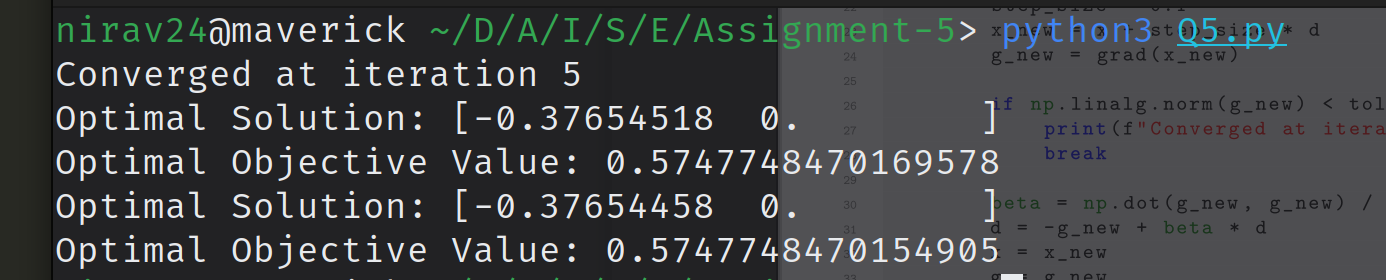
\includegraphics[width=0.8\textwidth]{Images/Q5.png}
\end{figure}

% \clearpage

\begin{question*}[6]
    Consider the following problem:

    \[
    \text{Minimize} \quad (x_1 - 5)^2 + (x_2 - 3)^2
    \]
    subject to 
    \[
    3x_1 + 2x_2 \leq 6,
    \]
    \[
    -4x_1 + 2x_2 + 2 \leq 4
    \]

    Formulate a suitable barrier problem with the initial parameter equal to $1$. Use an unconstrained optimization technique starting with the point \( (0, 0) \) to solve the barrier problem.
\end{question*}

\begin{lstlisting}[language=Python]
import numpy as np
from scipy.optimize import minimize

def objective(x):
    x1, x2 = x
    return (x1 - 5)**2 + (x2 - 3)**2

def barrier(x, mu):
    x1, x2 = x
    g1 = 6 - (3 * x1 + 2 * x2)
    g2 = 2 - (-4 * x1 + 2 * x2)
    
    if g1 <= 0 or g2 <= 0:
        return np.inf
    
    return -mu * (np.log(g1) + np.log(g2))

def barrier_objective(x, mu):
    return objective(x) + barrier(x, mu)

def solve_barrier_problem(mu, x0):
    result = minimize(barrier_objective, x0, args=(mu), method='CG', options={'disp': True})
    return result.x, result.fun

mu = 1
x0 = np.array([0.0, 0.0]) 

solution, objective_value = solve_barrier_problem(mu, x0)

print("Optimal Solution: ", solution)
print("Optimal Objective Value: ", objective_value)
\end{lstlisting}

\begin{question*}[7]
    Consider the following problem:

    \[
    \text{Minimize} \quad x_1^2 + 2x_2^2
    \]
    subject to
    \[
    2x_1 + 3x_2 - 6 \leq 0, \quad -x_2 + 1 \leq 0.
    \]

    \begin{enumerate}[label=(\alph*)]
        \item Find the optimal solution to this problem.
        \item Formulate a suitable function with an initial penalty parameter \( \mu = 1 \).
        \item Starting from the point \( \begin{bmatrix} 2 & 4 \end{bmatrix}^\top \), solve the resulting problem by a suitable unconstrained optimization technique.
    \end{enumerate}
\end{question*}

\begin{proof}        
    First, rewrite the constraints:

    \[
    g_1(x_1, x_2) = 2x_1 + 3x_2 - 6 \leq 0, \quad g_2(x_1, x_2) = -x_2 + 1 \leq 0.
    \]

    The Lagrange function for this problem is:

    \[
    \mathcal{L}(x_1, x_2, \mu_1, \mu_2) = x_1^2 + 2x_2^2 + \mu_1 (2x_1 + 3x_2 - 6) + \mu_2 (-x_2 + 1).
    \]

    The KKT conditions are:
    \[
    \nabla_{x_1} \mathcal{L} = 0, \quad \nabla_{x_2} \mathcal{L} = 0,
    \]
    along with the complementary slackness conditions:
    \[
    \mu_1 (2x_1 + 3x_2 - 6) = 0, \quad \mu_2 (-x_2 + 1) = 0.
    \]

    Solving these equations taking cases when $\mu_1$ is or is not $0$ and $\mu_2$ is or is not $0$, we get the optimal solution as $\begin{bmatrix} 0 & 1 \end{bmatrix}^\top$.

    Therefore, the optimal solution is:

    \[
    \mathbf{x}^* = \begin{bmatrix} 0 \\ 1 \end{bmatrix}.
    \]
\end{proof}

\begin{question*}[8]
    Consider the following problem:

    \[
    \text{minimize} \quad \frac{1}{2} \|\mathbf{x}\|^2
    \]
    \[
     \text{subject to} \quad A \mathbf{x} = \mathbf{b},
    \]
    where \( A \in \mathbb{R}^{m \times n}, m < n \) and \( A \) is full row rank. Show that if \( \mathbf{x}^{(0)} \in \{ \mathbf{x} : A \mathbf{x} = \mathbf{b} \} \), then the projected steepest descent algorithm converges to the solution in one step.
\end{question*}

\begin{proof}
    Let the objective function be:

    \[
    f(\mathbf{x}) = \frac{1}{2} \|\mathbf{x}\|^2 = \frac{1}{2} \mathbf{x}^\top \mathbf{x}.
    \]

    The gradient of \( f(\mathbf{x}) \) is (by \href{https://michael.orlitzky.com/articles/the_derivative_of_a_quadratic_form.xhtml}{derivative of quadratic form}):

    \[
    \nabla f(\mathbf{x}) = \mathbf{x}.
    \]

    The projected steepest descent algorithm iteratively updates the solution using the gradient direction and projects the result onto the feasible set defined by \( A \mathbf{x} = \mathbf{b} \).

    The update rule for the projected steepest descent method is:

    \[
    \mathbf{x}^{(k+1)} = \text{Proj}_{A\mathbf{x}=\mathbf{b}} \left( \mathbf{x}^{(k)} - \alpha_k \nabla f(\mathbf{x}^{(k)}) \right),
    \]
    where \( \alpha_k \) is the step size at the \( k \)-th iteration and \( \text{Proj}_{A\mathbf{x}=\mathbf{b}} \) denotes the projection onto the feasible set \( \{ \mathbf{x} : A \mathbf{x} = \mathbf{b} \} \).

    Since \( \mathbf{x}^{(0)} \) satisfies the constraint \( A \mathbf{x}^{(0)} = \mathbf{b} \), the starting point is already in the feasible set. The gradient at this point is:

    \[
    \nabla f(\mathbf{x}^{(0)}) = \mathbf{x}^{(0)}.
    \]

    The update step is:

    \[
    \mathbf{x}^{(1)} = \text{Proj}_{A\mathbf{x}=\mathbf{b}} \left( \mathbf{x}^{(0)} - \alpha_0 \mathbf{x}^{(0)} \right).
    \]

    If we choose \( \alpha_0 = 1 \) (the value which optimizes the objective function), the update becomes:

    \[
    \mathbf{x}^{(1)} = \text{Proj}_{A\mathbf{x}=\mathbf{b}} \left( \mathbf{x}^{(0)} - \mathbf{x}^{(0)} \right) = \text{Proj}_{A\mathbf{x}=\mathbf{b}} \left( \mathbf{0} \right).
    \]

    Thus, the projection of the origin \( \mathbf{0} \) onto the feasible set \( \{ \mathbf{x} : A \mathbf{x} = \mathbf{b} \} \) will give the point in the feasible set closest to the origin. This point is the optimal solution to the problem.

    Since the feasible set is defined by \( A \mathbf{x} = \mathbf{b} \), the projection of the origin \( \mathbf{0} \) onto this set is the solution \( \mathbf{x} \) that satisfies \( A \mathbf{x} = \mathbf{b} \). Hence, the projected steepest descent method converges to the optimal solution in one step.
\end{proof}

\end{document}